\PassOptionsToPackage{utf8}{inputenc}
\documentclass{bioinfo}
\copyrightyear{2020} \pubyear{2020}
\usepackage[colorlinks=true,urlcolor=black,citecolor=blue]{hyperref}
\access{Advance Access Publication Date: Day Month Year}
\appnotes{Manuscript Category}

\newcommand\st{\textbf{Stitcher}}
\newcommand\ix{\textbf{InXight Drugs}}

\begin{document}
\firstpage{1}

\subtitle{Database and ontologies}

\title[Stitcher: An entity resolution framework]{Stitcher: An entity resolution framework for comprehensive data integration of approved drugs}
\author[Nguyen \textit{et~al}.]{Dac-Trung Nguyen,$^{\text{\sfb 1}}$
Ivan Grishagin,$^{\text{\sfb 1}}$
Daniel Katzel,$^{\text{\sfb 1}}$
Tyler Peryea,$^{\text{\sfb 1,2}}$ and Noel Southall\,$^{\text{\sfb 1},\ast}$}
\address{$^{\text{\sf 1}}$Division of Pre-clinical Innovation, National Center for Advancing Translational Sciences (NCATS), National Institutes of Health, USA\\
$^{\text{\sf 2}}$Present address: Office of Health Informatics, Office of Chief Scientist, Food and Drug Administration, USA}

\corresp{$^\ast$To whom correspondence should be addressed.}

\history{Received on XXXXX; revised on XXXXX; accepted on XXXXX}

\editor{Associate Editor: XXXXXXX}

\abstract{\textbf{Motivation:}
\\
\textbf{Results:} Text  Text Text Text Text Text Text Text Text Text  Text Text Text Text Text
Text Text Text Text Text Text Text Text Text Text Text Text Text  Text Text Text Text Text Text\\
\textbf{Availability:} The complete source code along with data and build instructions for \st{} is readily available on Github \url{https://github.com/ncats/stitcher}. The \ix{} resource is accessible at \url{https://drugs.ncats.io}.\\
\textbf{Contact:} \href{mailto:southalln@mail.nih.gov}{southalln@mail.nih.gov}\\
\textbf{Supplementary information:} Supplementary data are available at \textit{Bioinformatics}
online.}

\maketitle

\section{Introduction}
As the volume of biological data continues to grow at an unprecedented rate, data de-duplication---also commonly known as record linkage or \emph{entity resolution}---is proportionally playing a prominent role in data integration. From the construction of training data for machine learning to building knowledge graphs as epistemological frameworks for artificial intelligence, proper entity resolution is essential in generating ground-truth data. The core challenge of entity resolution is in establishing \emph{uniqueness}. For well-defined entity types (e.g., gene, tissue, cell line), uniqueness is determined solely based on established identifiers and nomenclature; for other entity types (e.g., drug, disease, phenotype), however, uniqueness is not as well-established due to conceptual ambiguities in how entities are defined and represented. Take the disease entity type as an example. The discrepancy between the theoretical concept of ``disease entity'' from its clinical nosology \citep{Hucklenbroich14} is what makes disease entity resolution extremely challenging.

Herein we report on our recent data integration effort to build a comprehensive resource of drugs that have either been marketed or approved in the United States for human use. Such a resource is not only instrumental for drug repurposing but also serves as a valuable tool to further our understanding of the mechanistic properties of molecular targets \citep{Huang2019}. To the best of our knowledge, \ix{} is currently the most comprehensive resource of its kind. In the remainder of this paper, we discuss data integration challenges associated with drug data, conceptually as well as technically. This discussion serves as the backdrop for the development of \st, an entity resolution framework that we have developed to address the shortcomings of traditional approaches.

\subsection{What is a ``drug''?}
\begin{itemize}
\item Summarize from \citep{Huang2011}
\item Distinction between different drug classes (e.g., small molecule, monoclonal antibodies, etc.); cite ISO 11238?
\item Introduce concepts for active moiety, salt form, excipient, etc.
\end{itemize}

\subsection{When are two drugs equivalent? (or Drug identity and equivalence)}
\begin{itemize}
\item Layout the challenges in determining when two drugs are equivalent. This will depend on drug classes. For example, for small molecules, discuss salt forms, metals, and esters; for biologics, biosimilar; etc.
\item Discuss the different types of identifier; INN, USAN, IUPAC, InChI, CAS, UNII, PubChem, company code, etc. Also address the challenge on the evolution of the drug identifier from discovery (where stereochemistry can be ambiguous) to approval.
\end{itemize}

%\enlargethispage{12pt}

\section{Approach}

\subsection{Preliminary concepts}
The conceptual data model underlying \st{} is a \emph{multigraph}. Within this multigraph, a node can either be a \emph{stitch node} or \emph{data node}. Each data node represents a ``raw'' entity as ingested from the data source; its corresponding stitch node is a \emph{standardized} representation that is used for \emph{stitching}. An edge between two stitch nodes can either be a \emph{stitch key} (undirected) or \emph{relationship} (directed). A unique \emph{stitch value} is associated with each stitch key such that it forms a clique. Figure~\ref{fig:graph1} shows an instance of a connected component of a stitch multigraph with overlapping cliques.

A connected component in the stitch multigraph represents the basic unit of work for entity resolution. While the majority of connected components are of reasonable sizes (e.g., 20 to 50 stitch nodes), the real challenges center around effective strategies for handling very large connected components---or also commonly known as \emph{hairballs} \citep{Croset2015}. For example, the current version of the \ix{} resource has an hairball close to 30,000 stitch nodes spanning across 15 data sources. We discuss our strategies in detail for untangling through such an hairball in Section~\ref{sec:methods_er}.

The primary goal of entity resolution is to determine the number of unique entities in a connected component. These derived entities are represented as \emph{sgroup nodes} in the stitch multigraph. There can be multiple instances of sgroup nodes for any given set of stitch nodes, with each instance reflects a specific algorithmic strategy or version. Figure~\ref{fig:graph1} shows that there is only one unique entity as determined by the entity resolution algorithm for the given connected component.

\begin{figure}[!tpb]
\centerline{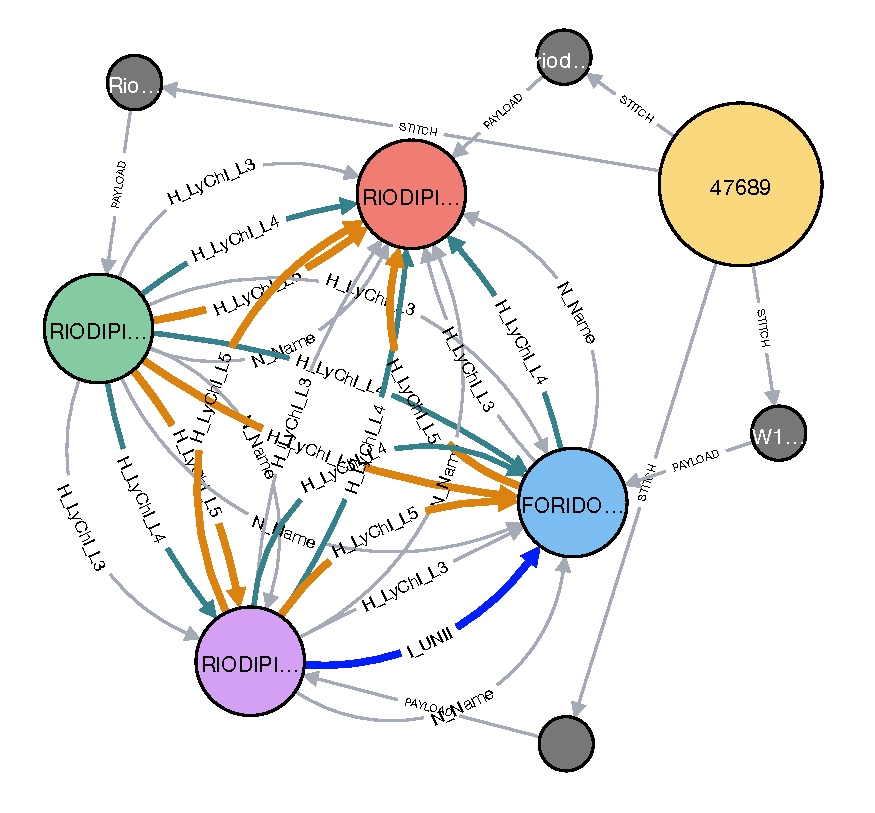
\includegraphics[scale=0.5]{graph3}}
\caption{A connected component in the stitch multigraph with four \emph{stitch nodes} (medium) and corresponding \emph{data nodes} (small). Each stitch value forms a clique within this connected component. The edge labels between stitch nodes are the stitch keys. The large node is the derived entity (i.e., sgroup node) generated from entity resolution.}\label{fig:graph1}
\end{figure}

\subsection{Stitch keys}
Stitch key is a core concept in \st. It defines how entities are matched, which, in turn, determines how cliques and connected components are formed. By virtue of its importance, the stitch key should reflect the true identity of the entity as much as possible. Depending on the entity type, the stitch key can be generic (e.g., synonym) or very specific (e.g., molecular hash key). For drug entity type, \st\ relies on the following stitch keys for each entity:
\begin{unlist}
\item{\texttt{N\_Name}.} This is the most generic stitch key available. Stitch values associated with this stitch key can be any established names or nomenclature; e.g., trade name, INN (International Nonproprietary Names), USAN (United States Adopted Names), IUPAC (International Union of Pure and Applied Chemistry).
\item{\texttt{I\_UNII}, \texttt{I\_CAS}, \texttt{I\_CODE}.} These stitch keys represent (i) unique identifiers assigned to the entity by a well-known registrar (e.g., the U.S. Food and Drug Administration in the case of UNII) or (ii) internal company code. Both \texttt{I\_UNII} and \texttt{I\_CAS} are specific to drug (or substance in general) entity type, whereas \texttt{I\_CODE} can be used for any type of identifiers. The decision to use specific stitch keys over generic ones ultimately rests on the strategies used within entity resolution.
\item{\texttt{H\_LyChI\_L5}, \texttt{H\_LyChI\_L4}, \texttt{H\_LyChI\_L3}.} For the small molecule class of drugs, perhaps more important than any identifiers is the underlying chemical structure definition. These stitch keys are hash values of the molecular structure at different resolutions \citep{lychi2019}.
\item{\texttt{R\_activeMoiety}.} Technically not a stitch key, the active moiety relationship between two drugs provides a strong evidence of equivalence. While this relationship can be infered directly from the chemical structures (e.g., freebase and salt forms, with and without esters), there is some level of curation needed to handle structures with metal complex.
\end{unlist}

\subsection{Data sources}
To build the \ix{} resource, \st\ currently utilizes 15 diverse data sources.

\subsection{Overall strategy}
The basic premise behind \st{} is that data integration is often done within the context of a specific data source. This is a reasonable assumption given the data quality varies when integrating across disparate sources. Futhermore, by establishing a reference data source for data integration, we have finer control over the following:
\begin{unlist}
\item{\emph{Data quality}.} A reference data source is typically selected such that it is of high quality. Here, we can also impose other data quality constraints (e.g., no synonyms can span multiple entities) to guide entity resolution.
\item{\emph{Data resolution}.} Entity resolution is particularly challenging when data integration involves ontologies. A reference data source can serve as the anchor ontology from which other ontologies can be mapped. As with data quality, we can also impose any additional semantic constraints; e.g., prostate cancer is not one of the diagnoses for a female patient in an electronic health record.
\item{\emph{Data curation}.} Generating ground-truth data is more managable with a single data source than across multiple data sources. This is particularly important due to the iterative feedback between data curation and data integration.
\end{unlist}

\begin{methods}
\section{Methods}\label{sec:methods}
In general, data integration with \st{} consists of four basic steps: \emph{ingestion}, \emph{stitching}, \emph{entity resolution}, and \emph{entity normalization}. With the exception of \emph{entity resolution}, all other steps---as they are currently implemented in \st---are generic and can be applied to a wide range of entity types.

\subsection{Data ingestion}
\st{} is capable of ingesting data in a wide variety of sources and formats. Semantic formats such as OWL, RDF, and Turtle are supported as are JSON, delimiter separated text, and custom formats. For non-semantic format, a separate configuration file is required to map properties to \emph{stitch keys}.

\subsection{Data stitching}

\subsection{Entity resolution}\label{sec:methods_er}

\subsection{Entity normalization}

%\enlargethispage{6pt}
\end{methods}

\section{Results}

%\begin{figure}[!tpb]%figure2
%%\centerline{\includegraphics{fig02.eps}}
%\caption{Caption, caption.}\label{fig:02}
%\end{figure}


\section{Discussion}


%%%%%%%%%%%%%%%%%%%%%%%%%%%%%%%%%%%%%%%%%%%%%%%%%%%%%%%%%%%%%%%%%%%%%%%%%%%%%%%%%%%%%
%
%     please remove the " % " symbol from %\centerline{\includegraphics{fig01.eps}}
%     as it may ignore the figures.
%
%%%%%%%%%%%%%%%%%%%%%%%%%%%%%%%%%%%%%%%%%%%%%%%%%%%%%%%%%%%%%%%%%%%%%%%%%%%%%%%%%%%%%%

\section{Conclusion}


\section*{Acknowledgements}

We thank our colleagues, Mark Williams and Tyler Beck, for their valuable proof-reading of early drafts of the manuscript. We also thank our colleague, Tongan Zhao, for his help in developing a prototype curation user interface for \st.

\bibliographystyle{natbib}
%\bibliographystyle{achemnat}
%\bibliographystyle{plainnat}
%\bibliographystyle{abbrv}
%\bibliographystyle{bioinformatics}
%
%\bibliographystyle{plain}
%
\bibliography{document}


\begin{thebibliography}{}
\bibitem[Croset \emph{et al}., 2015]{Croset2015}
Croset, S., Rupp, J., Romacker, M. (2016) Flexible data integration and curation using a graph-based approach, \emph{Bioinformatics}, \textbf{32(6)}, 918--925.

\bibitem[Huang \emph{et al}., 2019]{Huang2019}
Huang, R., Zhu, H., Shinn, P., Ngan, D., Ye, L., Thakur, A.,
Grewal, G., Zhao, T., Southall, N., Hall, M., Simeonov, A., Austin, C. (2019) The NCATS Pharmaceutical Collection: a 10-year update, \emph{Drug Discovery Today}, \textbf{12(24)}, 2341--2349.

\bibitem[Huang \emph{et al}., 2011]{Huang2011}
Huang, R., Southall, N., Wang, Y., Yasgar, A., Shinn, P.,
Jadhav, A., Nguyen, D-T., Austin, C. (2011) The NCGC Pharmaceutical Collection:
A Comprehensive Resource of Clinically Approved Drugs Enabling Repurposing and Chemical Genomics, \emph{Science Translational Medicine}, \textbf{80(3)}, 80ps16.

\bibitem[Hucklenbroich, 2014]{Hucklenbroich14}
Hucklenbroich, P. (2014) ``Disease Entity'' as the Key Theoretical Concept of Medicine, \emph{Journal of Medicine and Philosophy}, \textbf{39}, 609--633.

\bibitem[LyChI, 2019]{lychi2019}
\emph{Layered Chemical Identifier} (2019), \url{https://github.com/ncats/lychi}, accessed October, 2019.

% \bibitem[Bofelli {\it et~al}., 2000]{Boffelli03}
% Bofelli,F., Name2, Name3 (2003) Article title, {\it Journal Name}, {\bf 199}, 133-154.

% \bibitem[Bag {\it et~al}., 2001]{Bag01}
% Bag,M., Name2, Name3 (2001) Article title, {\it Journal Name}, {\bf 99}, 33-54.

% \bibitem[Yoo \textit{et~al}., 2003]{Yoo03}
% Yoo,M.S. \textit{et~al}. (2003) Oxidative stress regulated genes
% in nigral dopaminergic neurnol cell: correlation with the known
% pathology in Parkinson's disease. \textit{Brain Res. Mol. Brain
% Res.}, \textbf{110}(Suppl. 1), 76--84.

% \bibitem[Lehmann, 1986]{Leh86}
% Lehmann,E.L. (1986) Chapter title. \textit{Book Title}. Vol.~1, 2nd edn. Springer-Verlag, New York.

% \bibitem[Crenshaw and Jones, 2003]{Cre03}
% Crenshaw, B.,III, and Jones, W.B.,Jr (2003) The future of clinical
% cancer management: one tumor, one chip. \textit{Bioinformatics},
% doi:10.1093/bioinformatics/btn000.

% \bibitem[Auhtor \textit{et~al}. (2000)]{Aut00}
% Auhtor,A.B. \textit{et~al}. (2000) Chapter title. In Smith, A.C.
% (ed.), \textit{Book Title}, 2nd edn. Publisher, Location, Vol. 1, pp.
% ???--???.

% \bibitem[Bardet, 1920]{Bar20}
% Bardet, G. (1920) Sur un syndrome d'obesite infantile avec
% polydactylie et retinite pigmentaire (contribution a l'etude des
% formes cliniques de l'obesite hypophysaire). PhD Thesis, name of
% institution, Paris, France.

\end{thebibliography}
\end{document}
